%%%%%%%%%%%%%%%%%%%%%%%%%%%%%%%%%%%%%%%%%
% v1.0.0
% lab-report-template
%%%%%%%%%%%%%%%%%%%%%%%%%%%%%%%%%%%%%%%%%

\documentclass[twocolumn]{article}


\usepackage[utf8]{inputenc}
\usepackage[a4paper,
            bindingoffset=0.2cm,
            left=1cm,
            right=1cm,
            top=1cm,
            bottom=2cm,
            footskip=1cm]{geometry}

\usepackage{lipsum}
\usepackage[italian,english]{babel}

\usepackage{graphicx} % Required to include images
\usepackage[labelfont=sc]{caption} %DT$18/02/2021 caption style
\usepackage{float} %DT$03/01/2020 better image positioning
\usepackage{cuted} %DT$29/07/2022 allows writing over the whole page

\usepackage{braket} % DT$13/11/2021 qm symbols
\usepackage{enumerate} % Custom item numbers for enumerations
\usepackage{placeins} %DT$04/01/2020 \FloatBarrier 
\usepackage{color} % Required for custom colors
\usepackage{amsmath,amsfonts,stmaryrd,amssymb,theorem} % Math packages
\usepackage{siunitx} %DT$03/01/2021 symbols ex:\SI{50}{\micro\second}
\sisetup{range-phrase={\text{\ -\ }},
     input-decimal-markers={.}, 
     range-units = single,
     output-decimal-marker = {.},
     group-digits=false}

\usepackage{booktabs}

\newcommand{\reffig}[1]{Figure~\ref{#1}}
\newcommand{\reftab}[1]{Table~\ref{#1}}
\newcommand{\refeqn}[1]{Equation~\ref{#1}}
\NewDocumentCommand\mat{mmmm}{%
\text{$\begin{pmatrix}#1 & #2\\#3 & #4\end{pmatrix}$}%
}

%%%%%%%%%%%%%%%%%%%%%%%%%%%%%%%%%%%%%%%%%%%% COMMENTS COLORS %%%%%%%%%%%%%%%%%%%%%%%%%%%%%%%%%%%%%%%%
\usepackage{dsfont}
\usepackage{xcolor}
\usepackage{todonotes}
\usepackage{ulem}
\usepackage{listings}

% global

\definecolor{todoxcolor}{HTML}{11aa00}
\newcommand{\todox}[2]{{\color{todoxcolor}\sout{#1}#2}}
\renewcommand{\todox}[1]{\todo[color=todoxcolor!20, inline]{{\it TODO:} #1}}

\definecolor{UniPDcolor}{HTML}{9B0014}
\newcommand{\UniPD}[1]{\todo[color=UniPDcolor, inline]{{\color{white}{\it UniPD contribution:} #1}}}
\newcommand{\todoUPD}[1]{\todo[color=UniPDcolor!20, inline]{{\it TODO UniPD:} #1}}


% people

\definecolor{fedecolor}{HTML}{FEDEBE}
\definecolor{fedecolor2}{HTML}{ff7600}
\newcommand{\fede}[2]{{\color{fedecolor2}{(Fede:\sout{#1} #2})}}
\newcommand{\fedecom}[1]{\todo[color=fedecolor!40, inline]{{\it Fede:} #1}}

\usepackage{csquotes}

\usepackage[table]{xcolor}
\usepackage{tabularx}
\usepackage{booktabs}

%%%%%%%%%%%%%%%%%%%%%%%%%%%%%%%%%%%%%%%%%
%               HEADER
%%%%%%%%%%%%%%%%%%%%%%%%%%%%%%%%%%%%%%%%%
\title{
    \vspace{-1cm}
    \vspace{0.5cm}
    \textbf{Analog Circuits vs Digital Circuits}\\
}
\author{
    {Lorenzo Tomba}
}

\date{October 2026}

% Document begin
\begin{document}
\maketitle

%%%%%%%%%%%%%%%%%%%%%%%%%%%%%%%%%%%%%%%%%
%                 BODY
%%%%%%%%%%%%%%%%%%%%%%%%%%%%%%%%%%%%%%%%%

\section{Some case of study}

In order to understand how much is the digital and analog part in circuits, we can study some examples of modern chips from big companies.
For every chip we can try to undersand how much of it is digital and how much is analog.

\subsection{Apple M4}

The Apple M4 is a SoC used in some iPads and Macs, it is realized with 3nm technology and obviously is made by a smaller blocks that can be divided betwwen analog, digital or mixed signal, as we can see in fingure \ref{Image 1}. \cite{apple_m4_2024}

\begin{figure}[h]
    \centering
    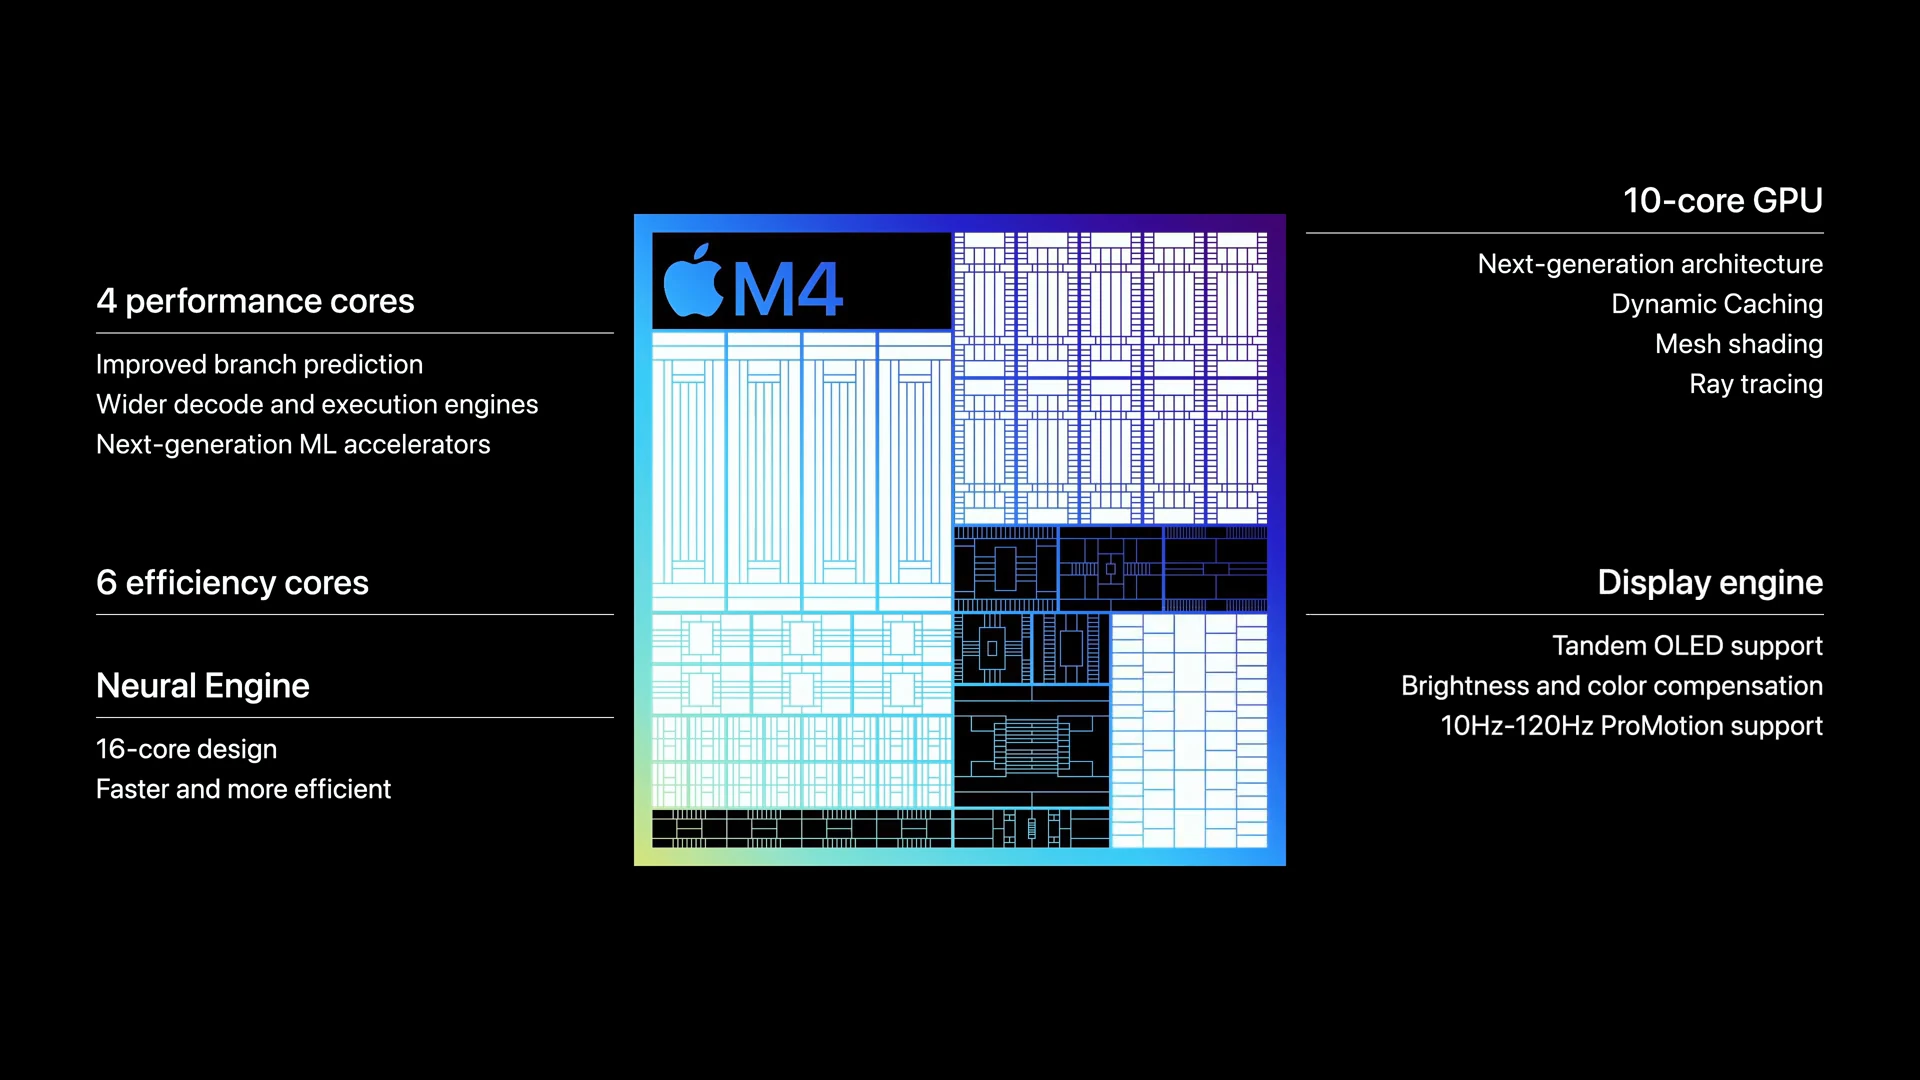
\includegraphics[width=.48\textwidth]{imgs/Apple_M4_simplified_schematic_parts.png}
    \caption{Apple M4 simplified schematic parts}
    \label{Image 1}
\end{figure}

Summuarizing the single blocks and making the separation we can consider the table \ref{tab:m4_blocks}.

\begin{table}[h]
    \centering    
    \begin{tabular}{p{0.62\columnwidth} p{0.25\columnwidth}}
        \hline
        \textbf{Apple M4 Integrated block} & \textbf{Classification} \\
        \hline
        CPU cores & Digital \\
        GPU cores & Digital \\
        Neural Engine & Digital \\
        CPU/GPU caches and SRAM & Digital \\
        Media Engine & Digital \\
        Image Signal Processor (ISP) & Mixed Signal \\
        Display engine & Digital \\
        Memory controllers & Mixed Signal \\
        Thunderbolt / USB controllers & Mixed Signal \\
        Clock generation and PLLs & Analog \\
        Power-management circuits & Analog \\
        High-speed I/O PHYs & Mixed Signal \\
        \hline
    \end{tabular}
    \caption{Functional classification of the main blocks of the Apple M4 SoC.}
    \label{tab:m4_blocks}
    \renewcommand{\arraystretch}{1.15}
\end{table}

\subsection{NVIDIA H100}

The NVIDIA H100 is another interesting example, it is a GPU used massivly for AI applications. We can see the simplified schematic in figure \ref{Image 2}. \cite{nvidia_h100_architecture_2022}

\begin{figure}[h]
    \centering
    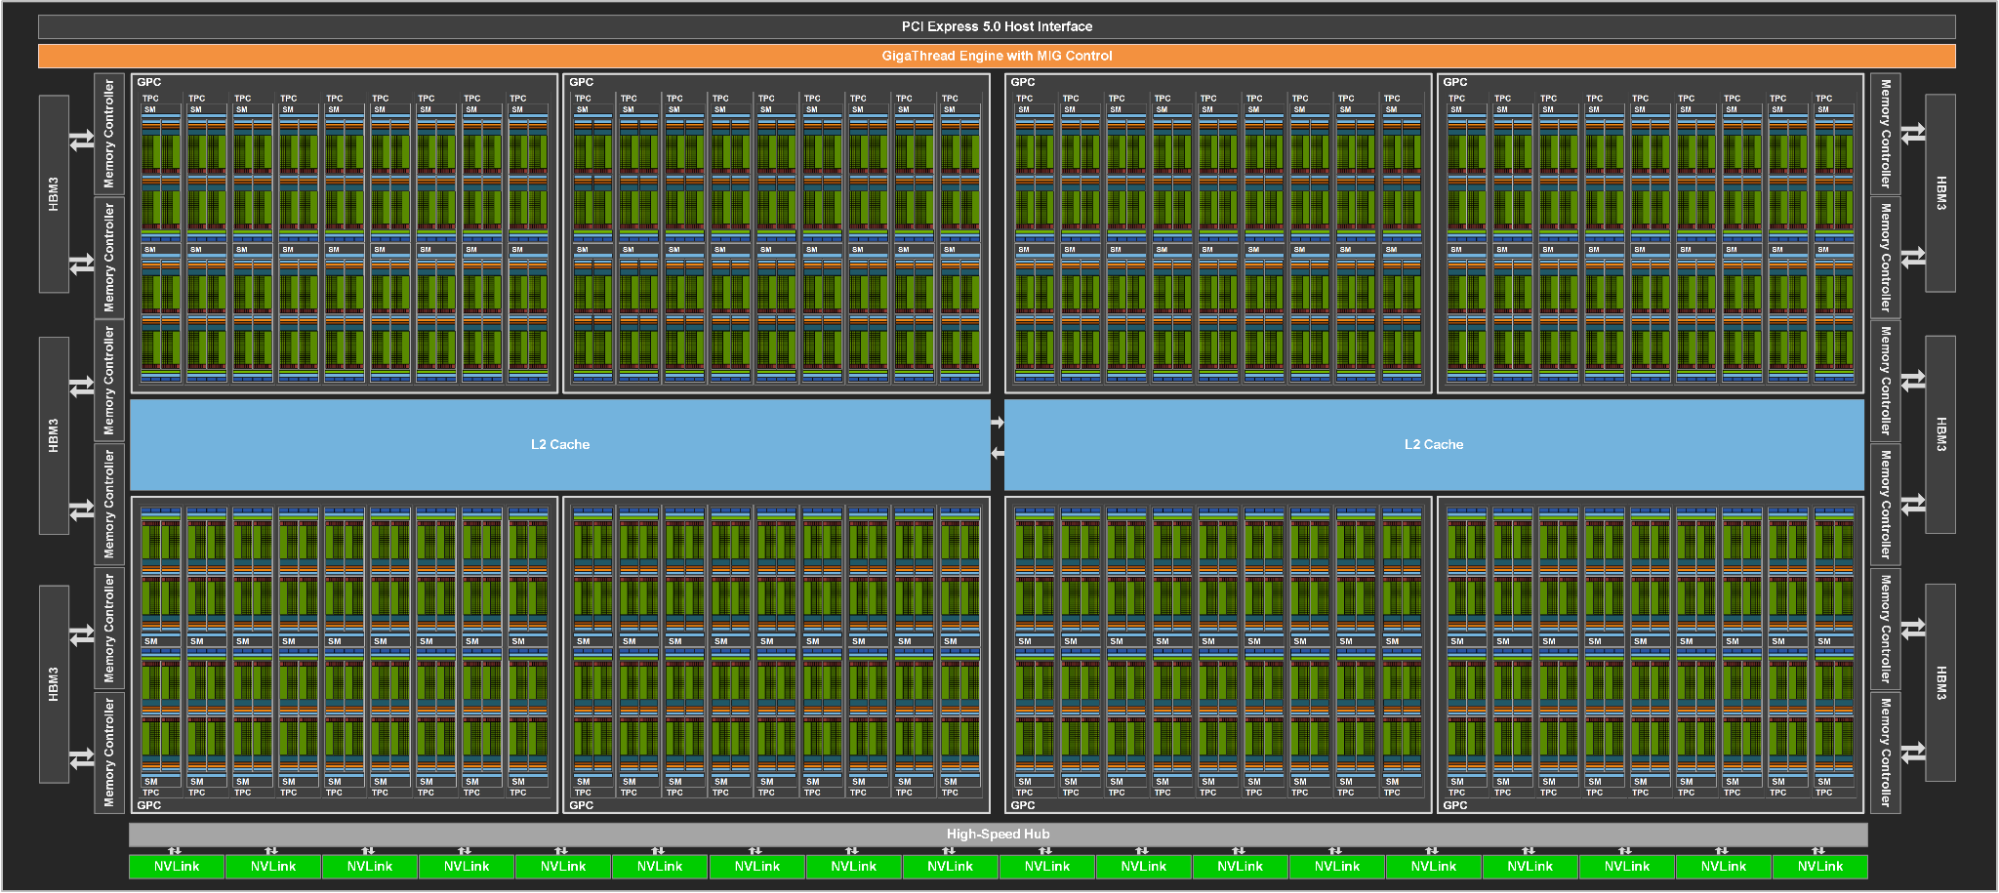
\includegraphics[width=.48\textwidth]{imgs/Full-H100-GPU-with-144-SMs.png}
    \caption{NVIDIA H100 simplified schematic parts}
    \label{Image 2}
\end{figure}

As before we can try to classify all the relevant blocks in order to understand the digital and anlog contibution on the chip. The data is shown in table \ref{tab:h100_blocks}. \cite{nvidia_hopper_2022}

\begin{table}[h]
    \centering
    \begin{tabular}{p{0.62\columnwidth} p{0.25\columnwidth}}
        \hline
        \textbf{NVIDIA H100 Integrated block} & \textbf{Classification} \\
        \hline
        Streaming Multiprocessors (SMs) & Digital \\
        CUDA cores & Digital \\
        Tensor Cores & Digital \\
        L1 cache and shared memory & Digital \\
        L2 cache & Digital \\
        Register files & Digital \\
        GPCs and GPU interconnect & Digital \\
        NVLink controllers & Mixed Signal \\
        HBM memory controllers & Mixed Signal \\
        PCIe interface & Mixed Signal \\
        Clock generation and PLLs & Analog \\
        High-speed I/O PHYs & Mixed Signal \\
        Power-management circuits & Analog \\
        \hline
    \end{tabular}
    \caption{Functional classification of the main blocks of the NVIDIA H100 GPU.}
    \label{tab:h100_blocks}
    \renewcommand{\arraystretch}{1.15}
\end{table}

\subsection{Snapdragon 8 Elite}

The Snapdragon 8 Elite is a SoC created by Qualcomm, ised in various smartphones. As the chips before we can divide the schematic in various blocks and classify them, as we can see in table \ref{tab:snapdragon_blocks}. \cite{qualcomm_snapdragon8elite_2024} \cite{qualcomm_snapdragon8elite_announcement_2024}

\begin{table}[h]
    \centering
    \begin{tabular}{p{0.62\columnwidth} p{0.25\columnwidth}}
        \hline
        \textbf{Snapdragon 8 Elite Integrated block} & \textbf{Classification} \\
        \hline
        Oryon CPU cores & Digital \\
        Adreno GPU & Digital \\
        Hexagon NPU & Digital \\
        Shared CPU cache & Digital \\
        AI accelerators & Digital \\
        Sensing Hub & Digital \\
        Spectra image signal processor & Digital \\
        Video processing engine & Digital \\
        Display processing & Digital \\
        Security processor & Digital \\
        5G modem baseband & Digital \\
        5G RF interface & Mixed Signal \\
        Wi-Fi / Bluetooth subsystem & Mixed Signal \\
        UWB interface & Mixed Signal \\
        High-speed memory interface & Mixed Signal \\
        Clock generation and PLLs & Analog \\
        Power-management circuits & Analog \\
        \hline
    \end{tabular}
    \caption{Functional classification of the main blocks of the Qualcomm Snapdragon 8 Elite SoC.}
    \label{tab:snapdragon_blocks}
    \renewcommand{\arraystretch}{1.15}
\end{table}

\section{Conclusion}
In conlusion, considering the three chips we can say that even if the chips showld be digital-based, still is needed a large amount of analog blcoks, for all three the chips.

%%%%%%%%%%%%%%%%%%%%%%%%%%%%%%%%%%%%%%%%%
%             BIBLIOGRAPHY
%%%%%%%%%%%%%%%%%%%%%%%%%%%%%%%%%%%%%%%%%
\bibliographystyle{plain}
\bibliography{references}

\end{document}